\documentclass[11pt,a4paper]{article}
\usepackage[T1]{fontenc}
\usepackage{amsmath,amssymb,graphicx,booktabs,geometry,fancyhdr,hyperref}
\geometry{margin=0.82in}
\hypersetup{hidelinks,pdfauthor={TEAM_NUMBER}}
\newcommand{\teamnumber}{\detokenize{TEAM_NUMBER}}
\pagestyle{fancy}\fancyhf{}\fancyhead[L]{\teamnumber}\fancyfoot[R]{\thepage}
\setlength{\headheight}{14pt}
\begin{document}
\begin{titlepage}\thispagestyle{fancy}\fancyfoot{}
\centering\vspace*{0.4in}
{\Large Problem B\par}\vspace{0.35in}
{\LARGE\bfseries What the First 0.10 Seconds Reveal About a Penalty Kick\par}\vspace{0.35in}
\begin{abstract}
Predicting a penalty kick from only two positions after launch is an inverse problem with six dynamical constraints. We compare analytic constant-acceleration extrapolation, a gravity-plus-drag fit, and an aerodynamic ensemble that marginalizes unresolved drag, density and spin. Independent Gaussian coordinate errors are sensitivity assumptions, not measured camera specifications. In 1000 synthetic kicks observed through 0.10 s with 0.01 m coordinate noise, paired goal-plane RMSEs are 1.07, 0.45 and 0.41 m, respectively; the ensemble nominal 95\% ellipse covers 94.6\% of airborne truths. For the supplied kick, the conditional ensemble mean is (y, z) = (3.08, 1.92) m at 0.396 s, and the most likely spatial location is approximately (3.21, 1.90) m. The joint 95\% ellipse has semiaxes 0.61 and 0.64 m; geometric center-point goal probability is 96.5\% under the stated prior. Unknown aerodynamics dominate conditional position noise. Longer observation reduces point error in an extended experiment, while undercoverage accompanies low effective sample sizes. Short observations support conditional probabilistic predictions rather than unique spin recovery; independent aerodynamic and tracking measurements remain necessary for field calibration.
\end{abstract}
\end{titlepage}
\section{Problem and information budget}
How much of a penalty trajectory is determined by its first 0.10 s? The target is the first forward crossing of the ball center through x = 11 m. The goal rectangle has -3.66 < y < 3.66 m and 0 < z < 2.44 m. The supplied positions are (0, 0, 0.11), (1.50, 0.45, 0.44), and (2.96, 0.86, 0.74) m at 0, 0.05 and 0.10 s, respectively. These are the official inputs, preserved without adjustment.\cite{upc2026}

With the initial position fixed, the later positions provide six scalar dynamical constraints. Initial velocity needs three parameters; unconstrained effective acceleration needs another three. Gravity plus an unknown drag coefficient and three spin components needs at least seven. An independent lift scale would add an eighth and create a spin-scale degeneracy. Thus a full aerodynamic inversion is structurally underdetermined. Counting all nine position coordinates while omitting the known initial state would overstate the information available.

A dimensionless local sensitivity calculation, scaling the velocity components by (30, 10, 10) m/s, drag by 0.25 and each spin component by 40 rad/s, confirms a six-by-seven matrix of rank six and a nontrivial null direction. These scales describe perturbations, not parameter error bars. The spin component parallel to velocity supplies no initial Magnus force. A unique numerical optimizer output therefore cannot establish a unique spin measurement. Three-dimensional aerodynamic coupling is essential even when its parameters remain uncertain.\cite{myers2013}

\section{A hierarchy of physical models}
Model 0 is a deliberately unconstrained baseline. For equally spaced observations with h = 0.05 s and displacement vectors d1 and d2 from the initial position, the effective velocity and acceleration are obtained analytically:

\begin{equation}
\mathbf{r}(t)=\mathbf{r}_0+\mathbf{v}_0t+\frac{1}{2}\mathbf{a}t^2,\qquad \mathbf{v}_0=\frac{4\mathbf{d}_1-\mathbf{d}_2}{2h},\qquad \mathbf{a}=\frac{\mathbf{d}_2-2\mathbf{d}_1}{h^2}.
\end{equation}
The supplied data give v0 = (30.4, 9.4, 6.9) m/s and a = (-16, -16, -12) m/s squared. These are short-window effective accelerations, not constant measured aerodynamic forces. The first forward root is selected; a later returning root is rejected. A negative discriminant or ground contact before the plane is retained as a no-point outcome.

\begin{equation}
t_g=\frac{2L}{v_{0x}+\sqrt{v_{0x}^2+2a_xL}},\qquad L=11\ {\rm m}.
\end{equation}
Models 1 and 2 use gravity and quadratic drag, with Model 2 additionally including a reduced Magnus term. In the following equations, r and v are position and velocity, omega is a constant angular-velocity vector, m is mass, A is cross-sectional area, rho is air density, R is ball radius, g is gravitational acceleration, and alpha is a fixed lift-law scale:

\begin{equation}
\frac{d\mathbf{r}}{dt}=\mathbf{v},\qquad \frac{d\mathbf{v}}{dt}=-g\mathbf{e}_z-k C_D|\mathbf{v}|\mathbf{v}+k\alpha R(\omega\times\mathbf{v}),\qquad k=\frac{\rho A}{2m}.
\end{equation}
Model 1 sets spin to zero and Cd to 0.25, fitting only three velocity components by nonlinear least squares. This isolates a low-variance physical constraint without pretending that drag was measured. Model 2 fixes alpha = 1 and treats drag, density and spin as nuisance parameters. Its linear lift relation is Cl = alpha R |omega|/|v|, with the cross product supplying the sine of the spin-velocity angle. Spin rate and an independent lift coefficient are never fitted simultaneously. Drag always opposes velocity, and the Magnus term performs no instantaneous work.

\begin{table}[htbp]\centering\small
\setlength{\tabcolsep}{3pt}
\begin{tabular}{p{0.205\linewidth}p{0.303\linewidth}p{0.383\linewidth}}\toprule
Quantity & Value or prior & Status\\\midrule
Mass; radius & 0.43 kg; 0.11 m & Representative choices within IFAB size/mass limits\\
Area; gravity & pi R squared; 9.81 m/s squared & Derived geometry; nominal local gravity\\
Density & Uniform 1.15-1.30 kg/m cubed & Assumed environmental sensitivity range\\
Drag coefficient & Uniform 0.12-0.40 & Assumed range, not ball-specific measurements\\
Spin magnitude; axis & Uniform 0-80 rad/s; isotropic & Assumed prior, not FIFA population statistics\\
\bottomrule\end{tabular}
\caption{Parameter provenance. Nominal density is 1.225 kg/m cubed; Model 1 uses nominal density. Every prior is an assumption.}
\end{table}
IFAB permits 410-450 g and circumference 68-70 cm; the selected mass and radius are representative values.\cite{ifab} Wind-tunnel studies show that drag depends on ball design and flow regime.\cite{asai2013} Published soccer-flight modeling uses comparable nominal mass, area and air density, but a punt-kick study does not calibrate an unknown penalty ball or our linear lift law.\cite{linthorne2011} The prior ranges in the table are consequently labeled assumptions, even where their scales are physically motivated.

Flight is integrated with fourth-order Runge-Kutta steps of 0.01 s. Synthetic truth uses 0.0025 s. Cubic Hermite interpolation and 36 bisections locate the first plane crossing or downward ground contact at z = R. Across three numerical probes, the maximum endpoint difference between 0.01 s and 0.00125 s integration was 2.5e-10 m, far below the measurement scenarios. Tests also recover constant velocity and the exact gravity-only parabola, verify force directions, and handle tangent launches with upward acceleration. No bounce is extrapolated through the ground.

\section{Prediction with unresolved aerodynamic parameters}
We assume independent, isotropic Gaussian coordinate noise on the two later positions and exact initial position and times. No camera specification is supplied, so sigma = 0.005, 0.01, 0.02 and 0.05 m are sensitivity scenarios. A central scenario of 0.01 m is used for detailed interpretation. These scales are not inferred from the residuals of six observations.

\begin{equation}
p(\mathbf{y}\mid\mathbf{v}_0,\eta,\sigma)\ \propto\ \exp\left[-\frac{\sum_{j=1}^2|\mathbf{r}(t_j;\mathbf{v}_0,\eta)-\mathbf{y}_j|^2}{2\sigma^2}\right].
\end{equation}
For each prior draw of nuisance parameters eta = (Cd, rho, omega), we minimize the six-coordinate squared residual over the three initial-velocity components. A broad, locally constant velocity prior has each component in [-60, 60] m/s and positive forward velocity. The conditional velocity posterior is integrated by a local Laplace approximation, rather than setting the fitted velocity to an exactly known value. If J is the six-by-three position Jacobian with respect to velocity, prior importance weights are:

\begin{equation}
w_i\ \propto\ \frac{\exp[-S_i/(2\sigma^2)]}{\sqrt{\det(J_i^{T}J_i)}},\qquad \sum_i w_i=1,\qquad N_{\rm eff}=\frac{1}{\sum_i w_i^2}.
\end{equation}
S\_i is the minimized residual sum of squares. Constants common to nuisance draws cancel. For each draw, we perturb the two observed positions with the assumed Gaussian noise, refit velocity conditionally, and propagate to the first event. This perturb-and-refit step approximates the local conditional state distribution; it is not a second likelihood update. We retain prior-averaged nuisance uncertainty and conditional state uncertainty together. Measurement-only propagation fixes representative nuisance parameters; nuisance-only propagation fixes the observed positions while retaining their likelihood. Those decompositions are conditional experiments, not additive causal variance components.

The posterior mean is the point estimate used for squared-error comparison. The most likely location is reported separately as a Gaussian-KDE grid mode, with Scott bandwidth scaling and stated grid resolution. Means, medians, covariance, marginal quantiles, event probabilities and effective sample sizes are saved. For a joint region, q95 is the weighted empirical 95th percentile of squared Mahalanobis distance, avoiding an untested Gaussian 5.99 threshold:

\begin{equation}
{\cal E}_{.95}=\{\mathbf{q}:(\mathbf{q}-\mu)^T\Sigma^{-1}(\mathbf{q}-\mu)\leq q_{.95}\},\qquad \mathbf{q}=(y_g,z_g).
\end{equation}
Location statistics condition on airborne plane crossing. Probability mass assigned to ground contact, no forward crossing or numerical failure is retained separately. Geometric goal probability uses the stated center-point rectangle; radius clearance instead uses |y| < 3.55 m and 0.11 < z < 2.33 m. Neither includes a goalkeeper, posts, net interaction, or rule-complete goal adjudication.

\section{General-method validation}
The main population contains 1000 independently generated kicks: speed uniformly 22-35 m/s, azimuth uniformly -22 to 22 degrees, elevation uniformly 5-18 degrees, and the stated nuisance distributions. These are synthetic design choices. The forward simulator generates full trajectories, but each estimator receives only the initial position and two noisy early positions. No future endpoint, true velocity, spin, drag or goal label enters inference. Methods use paired noisy observations; noise is scaled from the same standardized draws across the four noise scenarios. The fixed seed is 20261107.

There are 958 airborne true crossings and 42 ground-before-plane cases, all retained. Error is Euclidean distance in the y-z plane. We report coordinate MAE, radial RMSE, median and 95th-percentile error, physical no-point rate, numerical failure rate, geometric goal/miss accuracy, and region coverage. Paired RMSE uses cases where all three methods supply coordinates; no-point rates prevent hiding excluded failures. Classification uses every generated case, assigning ground-before-goal as a miss. An unavailable region on an airborne truth counts as uncovered.

\begin{equation}
E=\sqrt{(y_{\rm pred}-y_{\rm true})^2+(z_{\rm pred}-z_{\rm true})^2},\qquad {\rm RMSE}=\sqrt{\frac{1}{n}\sum_{i=1}^n E_i^2}.
\end{equation}
The main validation uses 512 nuisance particles per case; supplied-case uncertainty uses 10,000. A separate 1000-kick mismatch experiment saturates the linear lift response by dividing it by sqrt(1 + (spin ratio/0.25) squared), and changes drag by a speed-dependent factor 1 + 0.2 tanh((25 - speed)/5), with speed in m/s. These are declared stress-test laws, not independently measured aerodynamics. Matched-simulator validation checks internal calibration; the mismatch test checks only these two departures.

\section{Accuracy, failures and calibration}
\begin{table}[htbp]\centering\small
\setlength{\tabcolsep}{3pt}
\begin{tabular}{p{0.089\linewidth}p{0.125\linewidth}p{0.134\linewidth}p{0.125\linewidth}p{0.125\linewidth}p{0.160\linewidth}p{0.134\linewidth}}\toprule
Model & Mean (m) & Median (m) & 95th (m) & RMSE (m) & No point (\%) & Cost (ms)\\\midrule
M0 & 0.90 & 0.78 & 1.97 & 1.07 & 12.4 & 0.00037\\
M1 & 0.37 & 0.33 & 0.83 & 0.45 & 0.9 & 0.094\\
M2 & 0.35 & 0.30 & 0.76 & 0.41 & 0.0 & 88\\
\bottomrule\end{tabular}
\caption{At sigma = 0.01 m. All four error columns use the same 836 common cases. No-point rate uses all 958 airborne truths. Cost is measured batched CPU elapsed time per case, excluding generation of truth; it is not an optimized deployment benchmark.}
\end{table}
Model 2 has the lowest paired RMSE in the four tested noise scenarios; at 1 cm, its reduction relative to Model 1 is 9\%. Its model-specific median error is 0.31 m and its 95th-percentile error is 0.77 m. The coordinate MAEs are 0.23 m in y and 0.22 m in z. Goal/miss classification is 89.8\% over all kicks, versus 87.7\% for fixed drag and 71.2\% for the baseline.

The nominal 95\% ellipse covers 94.6\% of 958 airborne truths at 1 cm. This is a measured calibration result, not an assumed 95\% guarantee. No numerical particle failure was observed in the tested main population. Physical no-point outcomes are substantial for unconstrained acceleration and remain in the raw tables. At 5 cm the paired RMSEs are 0.505 m for fixed drag and 0.503 m for Model 2: this small descriptive difference does not establish a meaningful practical advantage, and classification is essentially tied.

\begin{figure}[htbp]\centering
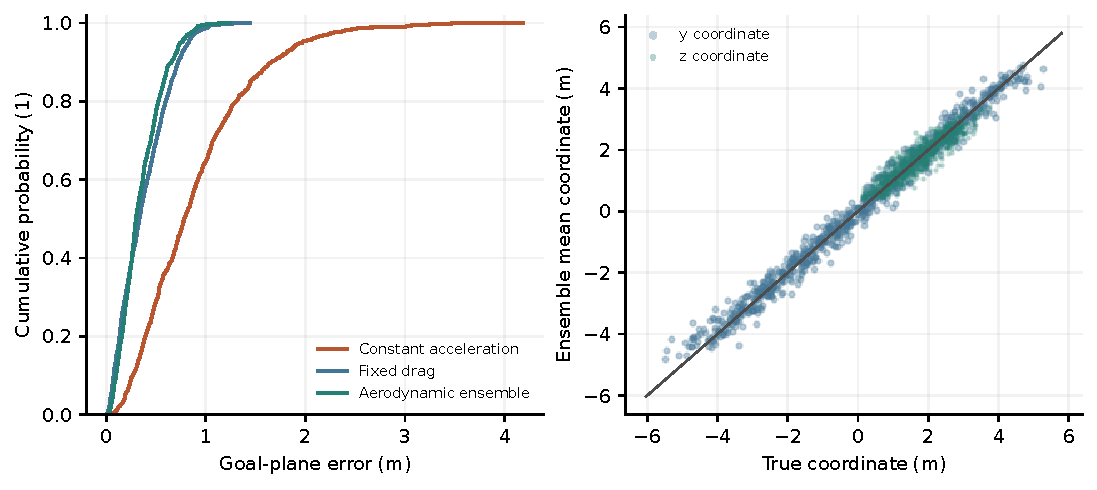
\includegraphics[width=\linewidth]{../figures/validation.pdf}
\caption{Paired synthetic errors at sigma = 0.01 m (left), and predicted versus true coordinates for Model 2 (right). Only common airborne coordinate cases enter this display; failure and classification denominators are reported separately.}
\label{fig:validation}
\end{figure}
\begin{figure}[htbp]\centering
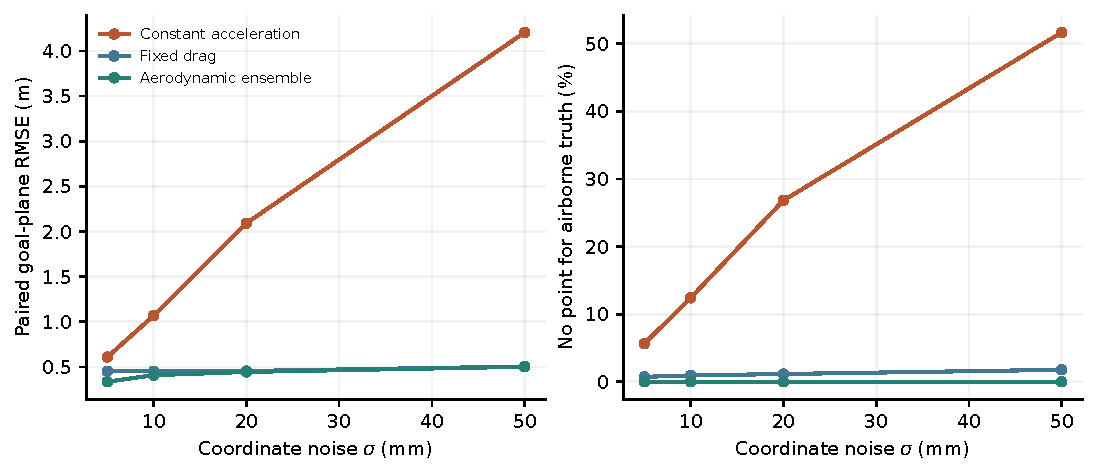
\includegraphics[width=\linewidth]{../figures/measurement_noise.pdf}
\caption{Noise dependence in the main synthetic population. Left: RMSE on common coordinate cases within each scenario, whose sample count changes with noise. Right: the proportion of airborne truths receiving no plane-coordinate prediction. No-point events include physically predicted ground contact and are distinct from numerical failures.}
\label{fig:measurement_noise}
\end{figure}
The mismatch population gives Model 2 paired RMSE 0.31 m and coverage 99.5\%. Lift saturation makes this particular population less strongly curved; therefore its smaller error is not evidence of general robustness. Coverage well above 95\% indicates conservative regions under this changed law. Unmodeled winds, drag crises and unsteady side forces could produce different errors.

\section{Prediction for the supplied kick}
\begin{table}[htbp]\centering\small
\setlength{\tabcolsep}{3pt}
\begin{tabular}{p{0.249\linewidth}p{0.285\linewidth}p{0.178\linewidth}p{0.178\linewidth}}\toprule
Model & Crossing time (s) & y (m) & z (m)\\\midrule
M0 & 0.405 & 2.49 & 1.92\\
M1 & 0.394 & 3.22 & 1.91\\
M2 mean & 0.396 & 3.08 & 1.92\\
M2 KDE mode & Not a joint time mode & 3.21 & 1.90\\
\bottomrule\end{tabular}
\caption{Deterministic M0/M1 intersections and Model 2 conditional posterior summaries at sigma = 0.01 m. A pointwise spatial mode is not assigned an invented most likely crossing time.}
\end{table}
The most likely spatial location is approximately (3.21, 1.90) m under the central scenario, while the squared-error-optimal posterior mean is (3.08, 1.92) m. The KDE grid spacing is approximately 2 cm in each direction, so its peak should not be interpreted more precisely. Mean crossing time is 0.396 s, with a 95\% interval of 0.381-0.410 s.

The marginal 95\% intervals are y = [2.56, 3.56] m and z = [1.43, 2.43] m. The joint 95\% ellipse has semiaxes 0.61 and 0.64 m; the two marginal intervals do not themselves form a joint 95\% rectangle. The covariance matrix, in square meters, is:

\begin{equation}
\Sigma=\left(\begin{array}{cc}0.0625 & -0.0004\\-0.0004 & 0.0561\end{array}\right)\ {\rm m}^2.
\end{equation}
The center-point in-goal probability is 96.5\%, and radius-clearance probability is 91.9\%. Their difference matters because the region approaches the crossbar and side boundary. The Monte Carlo standard error of the first probability is approximately 0.16 percentage points; it does not include prior or physical-model error. Effective sample size is 7017 of 10,000, with no noncrossing or numerical-failure mass in this scenario.

\begin{figure}[htbp]\centering
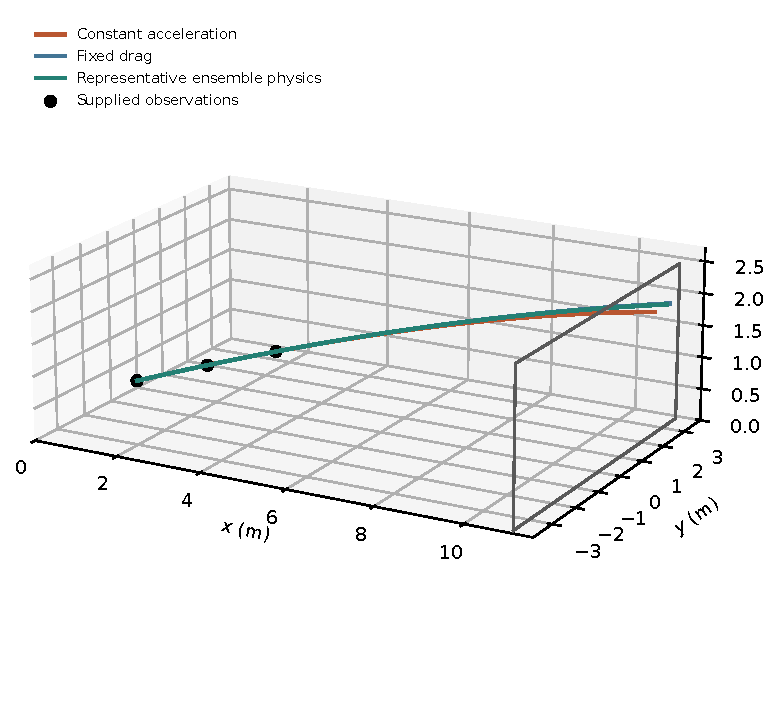
\includegraphics[width=\linewidth]{../figures/trajectory.pdf}
\caption{Supplied observations and extrapolations. Model 2 displays a trajectory using representative posterior nuisance parameters, rather than claiming that a trajectory through posterior means is itself the mean trajectory. The rectangle lies in the goal plane.}
\label{fig:trajectory}
\end{figure}
\begin{figure}[htbp]\centering
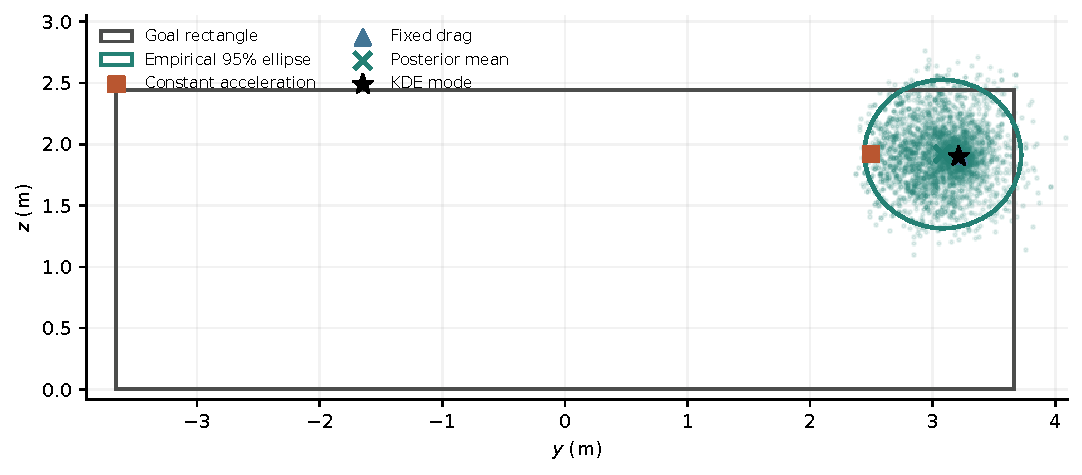
\includegraphics[width=\linewidth]{../figures/goal_plane.pdf}
\caption{Supplied-kick predictive distribution at sigma = 0.01 m. The cloud is a weighted resample for display; the ellipse is computed from the complete ensemble. The star denotes the KDE spatial mode, the cross the posterior mean. Portions outside the rectangle retain their miss probability.}
\label{fig:goal_plane}
\end{figure}
\section{Sensitivity, convergence and observation duration}
With representative nuisance parameters fixed, coordinate standard deviations from measurement noise alone are 0.034 and 0.033 m. With observations fixed, nuisance spread gives 0.25 and 0.23 m. Combined values are 0.25 and 0.24 m. Thus unresolved aerodynamics dominate this conditional scenario; the two components are not guaranteed to add exactly.

Changing only the assumed spin ceiling from 40 to 120 rad/s moves the supplied mean y from 3.17 to 2.98 m and the geometric goal probability from 100.0\% to 93.0\%. These are alternative priors, not competing measurements. Conditional sweeps of drag, density, spin rate, spin axis and lift scale, and population-bin analyses of speed and launch directions, are saved. Velocity perturbations are propagated separately to quantify how initial y/z motion affects the remote endpoint.

\begin{figure}[htbp]\centering
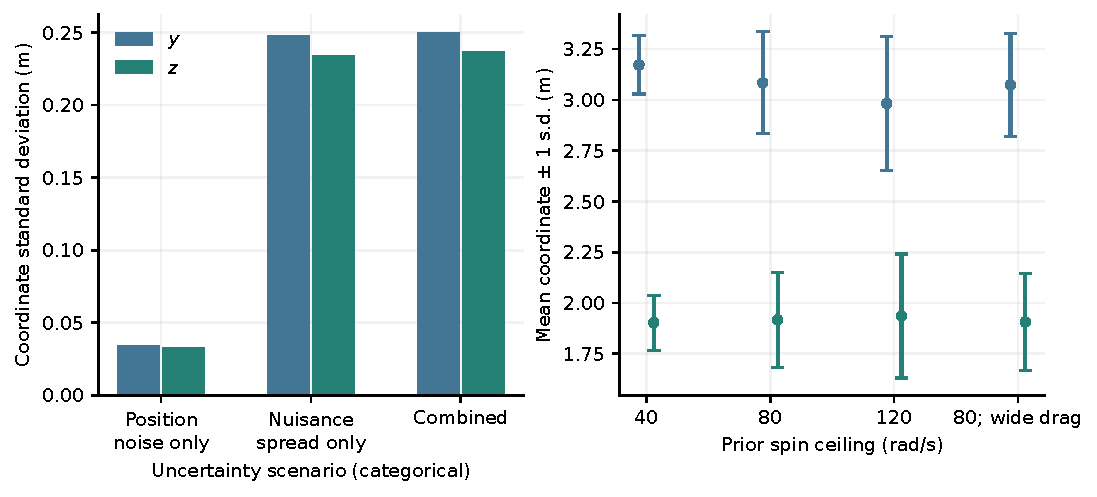
\includegraphics[width=\linewidth]{../figures/uncertainty_components.pdf}
\caption{Left: conditional uncertainty components; the bars are not an additive variance decomposition. Right: alternative prior scenarios with mean plus/minus one standard deviation, rather than 95\% error bars. The final scenario widens the drag prior as well.}
\label{fig:uncertainty_components}
\end{figure}
\begin{figure}[htbp]\centering
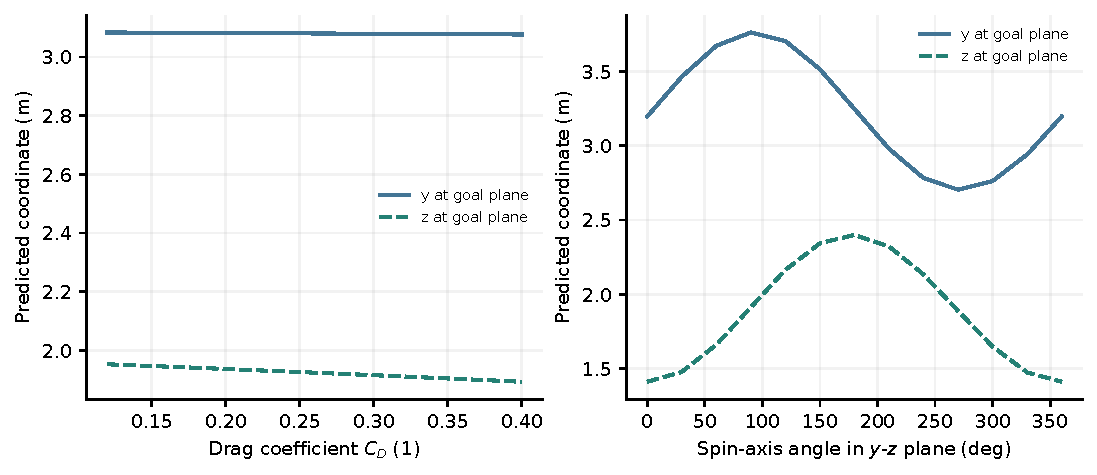
\includegraphics[width=\linewidth]{../figures/aerodynamic_sensitivity.pdf}
\caption{Endpoint sensitivity with the supplied observations held fixed and initial velocity refitted for each nuisance value. Right: a 50 rad/s spin vector rotates in the y-z plane. These are conditional model responses, not identified physical parameters.}
\label{fig:aerodynamic_sensitivity}
\end{figure}
Increasing supplied-case sampling from 1,000 through 5,000 to 10,000 changes the reported mean y from 3.089 to 3.088 to 3.083 m. Mean z remains approximately 1.92 m. The goal-probability range across these sample sizes is 96.33-96.62\%. This supports centimeter-scale stability of the central mean, not exact probability convergence.

In the 5 mm main-validation scenario, 40 cases have effective sample size below 30 with the frozen 512-particle budget. Refining every such case to 10,000 particles changes the mean coordinate prediction by at most 0.11 m; these diagnostic results are preserved separately and the frozen main comparison is unchanged. Low effective sample size is a computational limitation, not evidence of a precisely known spin.

The extended analysis uses 400 additional kicks and only two later observations at T/2 and T, with sigma = 0.01 m. It does not add observations to the original problem. Common-case Model 2 RMSE decreases from 0.50 m at T = 0.05 s to 0.18 m at T = 0.20 s. At 0.20 s, constant acceleration gives 0.22 m, better than the fixed-drag model at 0.34 m. This demonstrates that adding a physical constraint can increase prediction error when spin is omitted; RMSE alone does not separate bias and variance.

\begin{figure}[htbp]\centering
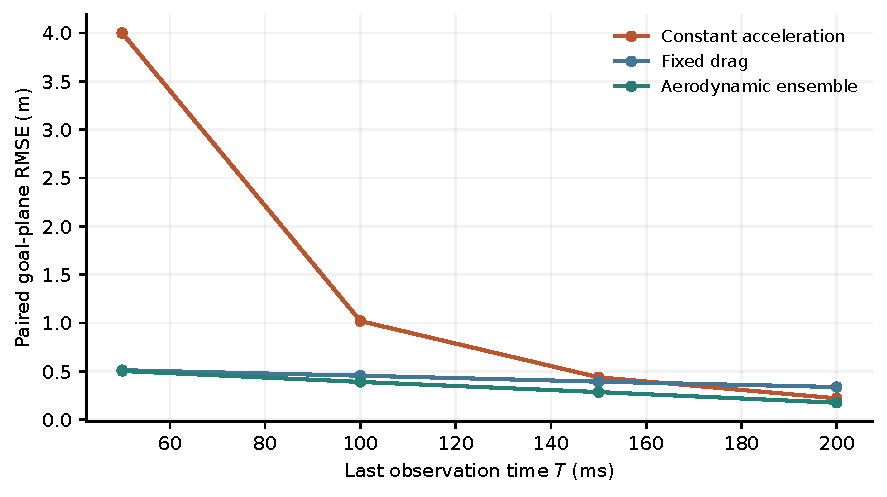
\includegraphics[width=\linewidth]{../figures/observation_duration.pdf}
\caption{Extended two-observation experiment, independent of the official supplied data. Common coordinate-case sets vary with duration. Longer observation improves these mean errors; it does not by itself validate goalkeeper reaction decisions or calibrated uncertainty.}
\label{fig:observation_duration}
\end{figure}
The extension uses 256 particles per case. At T = 0.20 s its nominal 95\% ellipse covers only 90.4\% of airborne truths, and the minimum effective sample size is 1.3. Narrower likelihoods challenge direct prior importance sampling. This undercoverage is retained as a failed calibration check; the extended results cannot justify a universal observation-time threshold for reliable goalkeeping. More efficient posterior sampling or substantially more particles would be needed before such a claim.

\section{Physical interpretation, strengths and limitations}
The baseline differentiates noisy coordinates twice. At fixed extrapolation time t, the coefficients of the two noisy positions are c1 = 2t/h - (t/h) squared and c2 = ((t/h) squared - t/h)/2. Coordinate uncertainty is therefore sigma sqrt(c1 squared + c2 squared), before accounting for uncertain crossing time. Acceleration noise grows as sqrt(5) sigma/h squared. This explains its steep noise sensitivity: effective curvature that exactly interpolates early positions is a noisy quantity, and exact interpolation supplies no residual check.

The physical models reduce this variance by restricting acceleration directions and magnitudes. Their gain depends on whether those restrictions describe the kick. Fixed drag cannot reproduce all sideways curvature, while an ensemble allows several nearly indistinguishable early trajectories to diverge by the goal. More physical free parameters would not create more observations. Averaging over unresolved parameters is a conditional uncertainty calculation, not a successful measurement of them.

Strengths are an explicit information budget, analytic baseline, physically signed forces, first-event root finding, retained misses and failures, paired general-method validation, uncertainty calibration tests, and numerical traceability. Every displayed numerical result and figure is generated from saved calculations. The single-command pipeline records its environment and uses no remote paid computation.

The dominant scientific limitation is the unmeasured aerodynamic prior and assumed lift law. The supplied ball, atmosphere, spin, tracking error and timing precision are unknown. Wind, spin decay, ball deformation, unsteady wake effects, drag crisis, camera bias and correlated errors are omitted. Initial position is treated as exact. Synthetic validation shares its main equations with inference, and the limited mismatch test is not field validation. The Laplace velocity approximation and low effective sample sizes limit some uncertainty estimates. No method here predicts goalkeeper motion or actual save probability. More trajectory points, calibrated cameras, measured spin and velocity, and independent flight tracks would reduce different parts of this uncertainty.

\section{Conclusion}
Two later positions constrain motion trends but do not uniquely recover drag and a spin vector. A conditional aerodynamic ensemble achieves paired RMSE 0.41 m and 94.6\% nominal-95\% coverage in the stated 1 cm synthetic scenario. For the supplied kick, the central-prior mean is (3.08, 1.92) m at 0.396 s; the KDE spatial mode is approximately (3.21, 1.90) m. The joint uncertainty spans roughly six-tenths of a meter in each principal direction. This conditional distribution, together with its prior dependence and calibration limitations, is more defensible than a purported unique spin reconstruction.

\clearpage
\bibliographystyle{unsrt}
\bibliography{references}
\section*{Report on the Use of AI}
OpenAI Codex was used for source lookup, modeling analysis, scientific programming, numerical experiments, plotting, English drafting and artifact checks. The exact underlying model identifier is not asserted. The scientific claims are limited to executed calculations and explicitly declared assumptions.

The official rules require the exact query and the complete AI output, in addition to naming the system.\cite{upcrules} The original project query is preserved verbatim in AI\_LOG.md and docs/original\_request.txt. Generated source files, numerical outputs and a visible-output archive document the assistance. This current research draft does not assert that a concise acknowledgment substitutes for the full required transcript. The complete exact input/output appendix must be reviewed and appended before contest submission. TEAM\_NUMBER remains a deliberate placeholder.

\end{document}
